暖气简化为一个以匀速在空间内上下移动的恒温热源。当外界温度及室内初始温度为10℃,室内设定温度为25℃时,通过\eqref{final equation}可以得出随时间变化的房间温度分布。

房间内某几个时刻的温度分布如下图所示:
\\
\begin{figure}[h]
    \centering
    \subfigure[空调刚开启时]{
    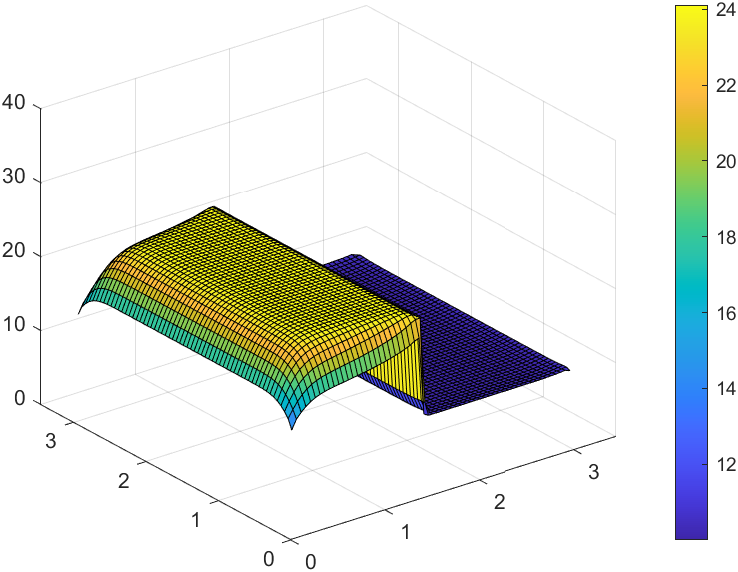
\includegraphics[width = 5.5cm]{figures/Nextroom-start.png}
    }\qquad
    \subfigure[空调向上扫风]{
    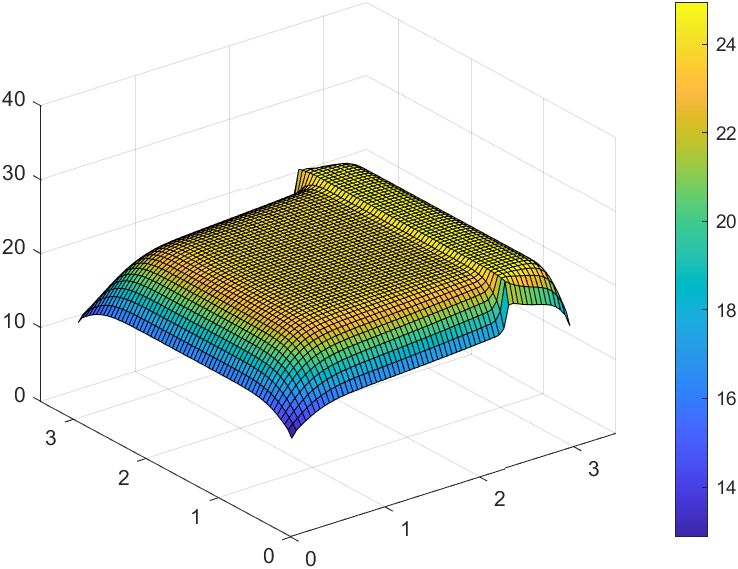
\includegraphics[width = 5.5cm]{figures/Nextroom-up.png}
    }\qquad
    \subfigure[空调向下扫风]{
    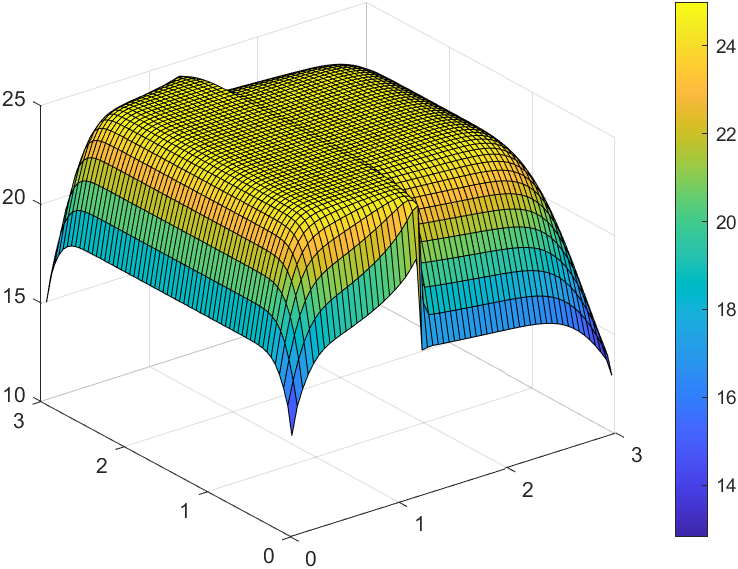
\includegraphics[width = 5.5cm]{figures/Nextroom-down.png}
    }\qquad
    \subfigure[房间竖直截面温度分布图]{
    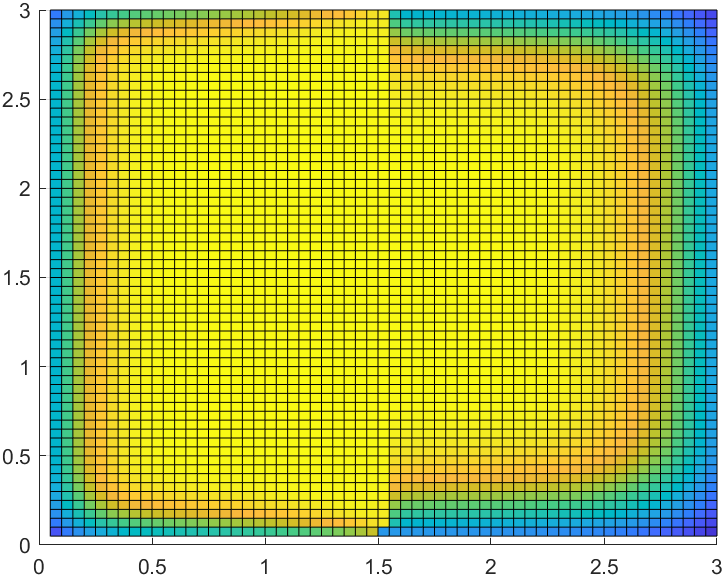
\includegraphics[width = 5.5cm]{figures/nextroom 2d.png}
    }\qquad
    
    \caption{隔壁房间开暖气时的温度分布}
    \label{隔壁房间开暖气时的温度分布}
\end{figure}


可以得到设置25℃空调时,室内的平均温度为23℃,墙边的平均温度为18℃。因此在研究待测房间的传热过程时将18℃作为边界条件。

